\documentclass[tikz,border=5pt]{standalone}

\usepackage{xcolor}
\usepackage{tikz}
\usetikzlibrary{shapes.geometric, arrows.meta, positioning}

\definecolor{azulp}{HTML}{1E4094}

\begin{document}

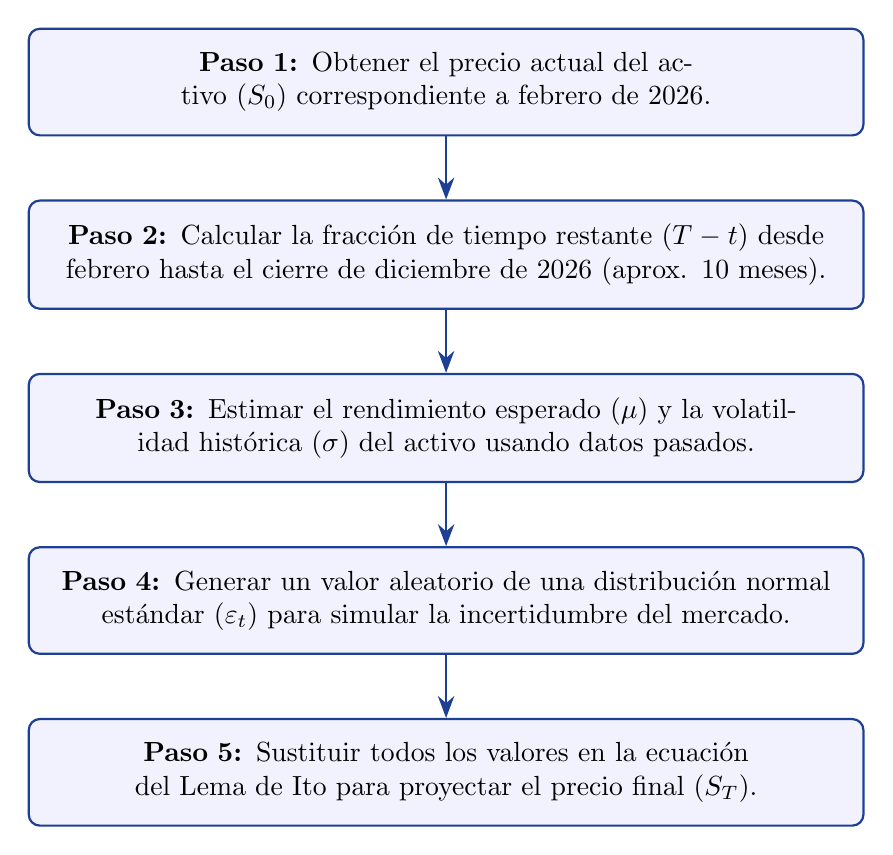
\begin{tikzpicture}[
    node distance=0.8cm and 0cm,
    caja/.style={rectangle, draw=azulp, thick, fill=blue!5, text width=10cm, align=center, rounded corners, minimum height=1cm, inner sep=0.3cm},
    flecha/.style={-{Stealth[scale=1.2]}, thick, azulp}
]

\node (paso1) [caja] {\textbf{Paso 1:} Obtener el precio actual del activo ($S_0$) correspondiente a febrero de 2026.};

\node (paso2) [caja, below=of paso1] {\textbf{Paso 2:} Calcular la fracción de tiempo restante ($T-t$) desde febrero hasta el cierre de diciembre de 2026 (aprox. 10 meses).};

\node (paso3) [caja, below=of paso2] {\textbf{Paso 3:} Estimar el rendimiento esperado ($\mu$) y la volatilidad histórica ($\sigma$) del activo usando datos pasados.};

\node (paso4) [caja, below=of paso3] {\textbf{Paso 4:} Generar un valor aleatorio de una distribución normal estándar ($\varepsilon_t$) para simular la incertidumbre del mercado.};

\node (paso5) [caja, below=of paso4] {\textbf{Paso 5:} Sustituir todos los valores en la ecuación del Lema de Ito para proyectar el precio final ($S_T$).};

\draw [flecha] (paso1) -- (paso2);
\draw [flecha] (paso2) -- (paso3);
\draw [flecha] (paso3) -- (paso4);
\draw [flecha] (paso4) -- (paso5);

\end{tikzpicture}

\end{document}